\chap{The Golden Angle}
This chapter is intended to give the reader a brief introduction to the golden ratio and its related mathematical concepts, followed by a brief overview of previous research in MRI with the golden-angle. Finally, a description of the novel methods developed as part of this thesis is presented.

\sect{The golden ratio}
If the ratio between two numbers, $a > b$, is equal to the ratio between the largest of the two and the sum of both, the ratio is called the golden ratio. This can be described as
\begin{equation}
    \label{eq:golden}
    \frac{a}{b} = \frac{a+b}{a} = \varphi
\end{equation}
and
\begin{equation}
    \label{eq:golden2}
    \frac{a+b}{a} = 1 + \frac{b}{a} =
    1 + \frac{1}{a/b}
\end{equation}
Combining Eq.~\ref{eq:golden} and \ref{eq:golden2} yields
\begin{equation}
    \label{eq:golden3}
    \varphi =
    1 + \frac{1}{\varphi}
\end{equation}
The golden ratio $\varphi$ has a few interesting properties. We sometime want to consider its conjugate
\begin{equation}
    \label{eq:conjugate_golden}
    \phi = \frac{1}{\varphi} = 1 - \varphi
\end{equation}
This kind of recursive formula is know as a continued fraction. On a general form, a continued fraction can be written as
\begin{equation}
    \label{eq:contf}
    a + \frac{1}{b + \frac{1}{c + ...}}
\end{equation}
where $a,b,c,...$ are known as partial quotients. An infinite continued fraction can be approximated by its convergents, i.e. what is left i the the recursion is stopped at any given point. If we write the 4 first convergent fractions on simplified form, we end up with
\begin{equation}
\label{eq:quotients}
a, \frac{1+ab}{b}, \frac{a+(1+ab)c}{1+bc}, \frac{1+ab+(a+(1+ab)c)d}{b+(1+bc)d}
\end{equation}
From Eq.\ref{eq:golden3} it's clear that $a = b = c = d = ... = 1$. Substitution yields
\begin{equation}
\label{eq:quotients2}
\frac{1}{1}, \frac{2}{1}, \frac{3}{2}, \frac{5}{3}
\end{equation}
Keeping on in a similar fashion will yield
\begin{equation}
\label{eq:quotients3}
\frac{5}{3}, \frac{8}{5}, \frac{13}{8}
\end{equation}
from Eq.~\ref{eq:quotients2} and \ref{eq:quotients3} we can see that the rational estimation of the golden ratio is in fact the fraction of two successive Fibonacci numbers. By taking the limit of the ratio of successive Fibonacci numbers at infinity we arrive at the golden ratio
\begin{equation}
    \lim_{n\to\infty} = \frac{F_n}{F_{n+1}} = \phi
    \label{eq:limit0}
\end{equation}
where $F_n$ denotes the nth Fibonacci number.

\sect{The golden angles}
There exist several ways to calculate an angle based on the golden ratio. Perhaps the most straight-forward would be to calculate the angle which divides the circle in two parts, where the ratio of the two central angles is the golden ratio
\begin{equation}
360^\circ \cdot \phi = 222.49^\circ  
\end{equation}
\begin{equation}
360^\circ \cdot (1 - \phi) = 137.51^\circ  
\label{eq:large_golden}
\end{equation}
However, it could be useful to only divide the half-circle, resulting in
\begin{equation}
\label{eq:large_ga}   
180^\circ \cdot \phi = 111.25^\circ  
\end{equation}
\begin{equation}
\label{eq:small_ga}
180^\circ \cdot (1 - \phi) = 68.754^\circ  
\end{equation}
Out of these four angles, Eq.~\ref{eq:large_ga} is the golden angle commonly used in MRI~\cite{Winkelmann2007}, whereas the angle defined by Eq.~\ref{eq:small_ga} is sometimes referred to as the small golden angle.

\sect{Multidimensional golden means}
The concept of the golden ratio can also be extended to higher dimensions~\cite{Anderson1993}. Two so called multidimensional golden means $\phi_1 = 0.4656$ and $\phi_2 = 0.6823$ are commonly used. The inverse $1/\phi_2 = 1.4656$ is the fourth smallest of the Pisot-numbers~\cite{Berestovskii2007}, and is sometimes known as the ``super-golden ratio''. It's has been proposed to enable three-dimensional golden-angle imaging~\cite{Chan2009, Trotier2015, Holst2017, Schrauben2020} by mapping the two golden-angles to a two-dimensional unit square
\begin{equation}
    x = \textrm{mod}(m\psi_1,1), y = \textrm{mod}(m\psi_2,1)
    \label{eq:double_golden_square}
\end{equation}
followed by a equal-area mapping of the unit square to a hemisphere
\begin{equation}
    \alpha = 2\pi\cdot x, \beta = \cos^{-1}(y)
\end{equation}
where $\alpha$ is the azimuthal angle and $\beta$ the the polar angle~\cite{Chan2009}.

\sect{Generalized golden angles}

\subsect{Pseudo-golden angles}
The golden-angle is approximately optimal for an arbitrary number of angles, as each succeeding angle of the series divides one of the largest gaps by the golden ratio. However, the number of readout lines are not always unknown at the beginning of the acquisition. Therefore, it would sometimes be useful to adapt the angle to be optimal for a specific number of spokes. This can be achieved in one of two ways. Either, the interval to be measured ($\pi$ or $2\pi$) is divided by a given number of lines, resulting in a so-called linear radial ordering, or by calculating the ``pseudo golden angle'' for the given number of lines~\cite{Svedin2018}.

\subsect{An existing generalization in 2D}
By restating eq.~\ref{eq:golden3}
\begin{equation}
    \phi = \frac{1}{1 - 1 + \frac{1}{\varphi}}
\end{equation}
together with eq.~\ref{eq:conjugate_golden} we note that
\begin{equation}
    1 - \phi = \frac{1}{2 - 1 + \frac{1}{\varphi}}
\end{equation}

It turns out that there exists an infinite series of ratios that have approximately golden properties~\cite{Wundrak2015}. The Nth generalized conjugate golden ratio can be derived through a simple geometric construction
\begin{equation}
\label{eq:general}
    \phi^N = \frac{1}{N-1+\frac{1}{\varphi}}
\end{equation}

This can be seen as a generalized Fibonacci series, $G^N(n+2) = G^N(n+1) + G^N(n)$, for $n \leq 0$ with initial conditions $G^N(0) = 0, G^N(1) = 1, G^N(2)$. By taking the limit of the ratio of the series as $n$ approaches infinity
\begin{equation}
    \lim_{n\to\infty} = \frac{G_n^1}{G_{n+1}^N} = \phi^N
    \label{eq:limit}
\end{equation}

By combining Eq.~\ref{eq:golden3} and Eq.~\ref{eq:general} it is evident that this is a continued fraction where all partial quotients except the first is one, meaning that regardless of N, all of these generalized golden means will be approximately as hard to estimate as a fraction of rational numbers as the original golden ratio.

\subsect{A novel generalization in 3D}
In this thesis, a novel generalization of the double golden angles was proposed, based on a similar construction as in the two-dimensional case.

It is based on the observation that, similar to Eq.~\ref{eq:limit}, the double golden angles can be constructed through a similar generalized Fibonacci series, $H^N(n+3) = H^N(n+2) + H^N(n)$ for $n \leq 0$ with initial conditions $H^N(0) = 0, H^N(1) = 1, H^N(2) = N$ at the limit

\begin{equation}
        \lim_{n\to\infty} = \frac{H_n^1}{H_{n+1}^N} = \phi^N_1 \quad \textrm{and} \quad \lim_{n\to\infty} = \frac{H_n^1}{H_{n+2}^N} = \phi^N_2
\end{equation}

will yield the original multidimensional golden means for N = 1, and for $N \geq 2$ will generate golden means with similar properties to the original golden means.

A geometric construction, similar to Eq.~\ref{eq:general} is also possible in 3D, and can be describes as
\begin{equation}
    \psi^N_2 =  \frac{1}{N - 1 + \frac{1}{\psi_2}} \quad \textrm{and} \quad \psi^N_1 = \frac{\psi^N_2}{1 + \psi_1}
\end{equation}
where $\psi_1$ and $\psi_2$ are the two original golden means. This is further discussed in Study II.

\sect{Golden angle in the literature}
The golden angle have found many uses within the field of MRI since the seminal paper was published in 2007~\cite{Winkelmann2007}. Many early adaptations were focused on dynamic contrast-enhanced (DCE) \Nomenclature{DCE}{Dynamic contrast enhancement} of chest and abdominal lesions~\cite{Lin2008}, breast MRI~\cite{Chan2009} and angiography~\cite{Prieto2010}. However, the golden-angle has found uses in many diverse areas, such as T1-mapping~\cite{Ehses2013, Tran-Gia2015} and diffusion weighted imaging~\cite{Seo2014}. In the field of cardiac MRI, the golden angle has been used for tissue phase mapping~\cite{Paul2016, Paul2016b}, imaging of arrhythmia~\cite{Contijoch2017}, determining pressure-volume loops~\cite{Witschey2014}, myocardial perfusion imaging~\cite{Sharif2014}, and measurement of respiratory induced variations in left-ventricular volumes~\cite{Holst2017, Holst2018, Holst2019}.

Arguably, the most successful method is Golden Angle Radial Sparse Parallel MRI (GRASP) \Nomenclature{GRASP}{Golden Angle Radial Sparse Parallel MRI}. It is a framework for dynamic contrast enhanced liver imaging~\cite{Feng2014}, which has been expanded with self-gating capabilities to the extra-dimensional GRASP (XD-GRASP) framework~\cite{Feng2015} for resolving multiple, and arbitrary temporal dimensions at once, such cardiac time and respiratory time~\cite{Feng2018}. The XD-GRASP formulation is based on the idea of a Sparse-SENSE~\cite{Feng2013}, which is based on an iterative SENSE reconstruction~\cite{Pruessmann2001} that is regularized by multiple sparse constraints~\cite{Lustig2007}. The general formulation can be described as a minimization problem on the form

 \begin{equation}\label{eq:argmin}
	\hat{\textbf{x}} = \argmin_{\textbf{x}} \|\textbf{y} - \textbf{E}\textbf{x} \|^2_2 + \lambda_1 \|\Psi_1\textbf{x}\|_1 + \lambda_2 \|\Psi_2\textbf{x}\|_1 + \dots + \lambda_N \|\Psi_N\textbf{x}\|_1
\end{equation}

where $\textbf{x}$ is the image, $\textbf{y}$ is the measured data, $\textbf{E}$ is the SENSE operator which includes the gridding step, Fourier transform and the coil sensitivities~\cite{Pruessmann2001}, $\Psi_N$ is the sparsifying transform in the Nth dimension~\cite{Lustig2007} and $\lambda_N$ controls the amount of regularization in the Nth dimension.

Another recent development making use of the golden-angle is the so-called MR multitasking method~\cite{Christodoulou2018, Shaw2019}, which uses a golden-angle readout with an integrated one-dimensional projection navigator and low-rank tensor decomposition to enable multiple simultaneous parameter mapping.

Other golden angle based methods may use the golden angle indirectly, e.g., for rotating spiral interleaves by the golden angles, often Eq.~\ref{eq:large_golden} to cover a full $360^\circ$ is commonly used~\cite{Kim2011}, or the ``spiral phyllotaxis'' method~\cite{Piccini2011, Piccini2017, Coppo2015}, which is a 3D-radial method based which traces Fibonacci spirals on the surface of the trajectory sphere, and where each interleave is rotated by the golden angle. The spiral phyllotaxis method has been used to enable fully respiratory and cardiac self-gated acquisitions~\cite{DiSopra2019}.

\sect{SWIG-PC}
In Study III, a novel phase-contrast pulse sequence was developed using a sector-wise golden-angle profile ordering~\cite{Han2016}, symmetric velocity encoding~\cite{Bernstein1992}, and a shared velocity encoding reconstruction~\cite{Bernstein1994, Lin2012}, to effectively double the number of reconstructed image frames. We decided to name this particular sequence ``Sector-wise golden-angle phase contrast'' or SWIG-PC for short. 

The golden-section division is performed according to the formula
\begin{equation}
    \phi_{n+1} = \textrm{mod} \left[ \left( \phi_n + \frac{\pi}{N} \cdot \frac{\sqrt{5}-1}{2} \right), \frac{\pi}{N} \right] + s \cdot \frac{\pi}{N}
\end{equation}
adapted from~\cite{Han2016}, where $s = 0, 1, 2, \dots, N$ denotes the current heartbeat, N is the total heartbeats to acquire and $\phi_n$ the $n$th angle, see Figure~\ref{fig:swig_overview}.

\begin{figure}
    \centering
    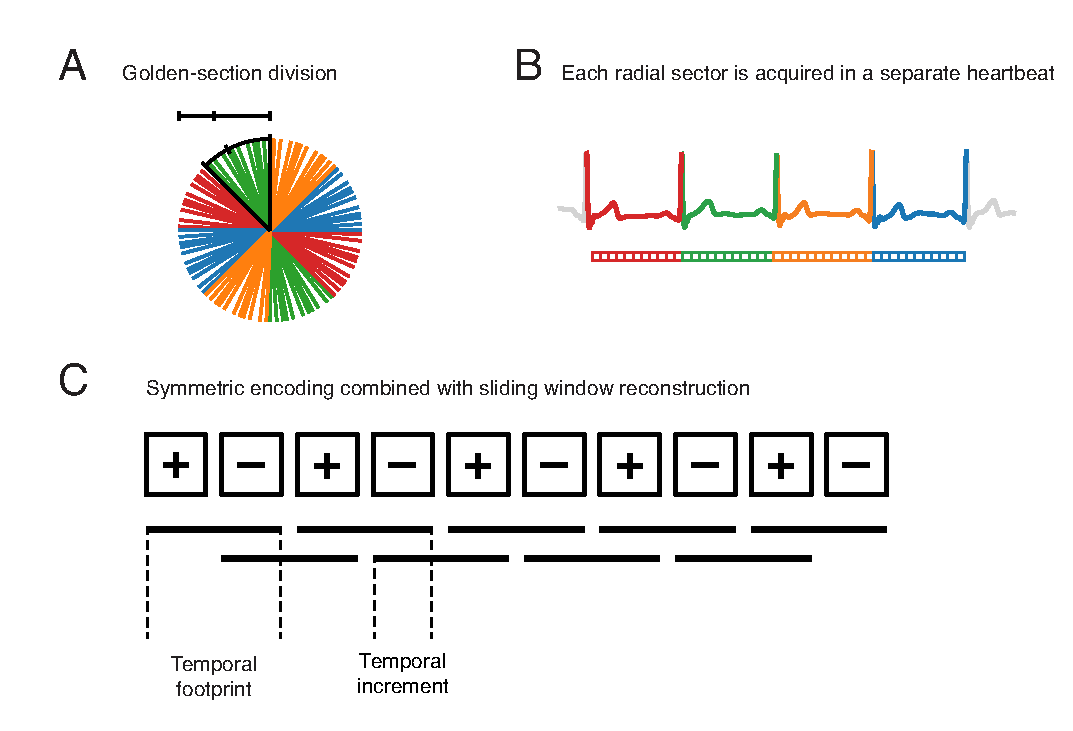
\includegraphics[width=\textwidth]{Figure_1_schematic_description}
    \caption{Schematic description of the SWIG-method. The k-space is sampled sector-wise with golden-section division within a sector of k-space (A). On each heartbeat, the acquisition moves to a new sector (B). Upon reconstruction, shared velocity encoding is used to double the reconstruction frames by performing phase subtraction between alternating positively- and negatively velocity encoded images. Reproduced with permission from~\cite{Fyrdahl2020}. (Licensed under CC BY 4.0) }
    \label{fig:swig_overview}
\end{figure}

The sector-wise golden angle profile ordering was combined with a TR-interleaved symmetric velocity encoding, to enable high temporal resolution phase contrast. This was applied to measuring diastolic dysfunction parameters in \textbf{Study II}.

\sect{3D-SWIG}
In Study IV, further development of the SWIG-PC method proposed in Study III was proposed. Instead of using phase contrast, we opted for functional imaging using bSSFP contrast. We decided to call the novel development ``3D Sector-wise golden angle'' or 3D-SWIG, for short.

Instead of mapping angles to a circle sector, as in SWIG-PC, polar coordinates were mapped to solid angles on a hemisphere. To enable a low distorting, uniform mapping, a method for constructing spherical grids~\cite{Rosca2011}, adapted to map coordinates from a cube to a sphere, see Figure~\ref{fig:mapping}. The resultant transform can be described as

\begin{equation}
    X' = x \cdot \sqrt{1-\frac{y^2}{2}-\frac{z^2}{2}-\frac{y^2z^2}{2}}
\end{equation}
\begin{equation}
    Y' = y \cdot \sqrt{1-\frac{z^2}{2}-\frac{x^2}{2}-\frac{z^2x^2}{2}}
\end{equation}
\begin{equation}
    Z' = z \cdot \sqrt{1-\frac{x^2}{2}-\frac{y^2}{2}-\frac{x^2y^2}{2}}
\end{equation}

Using this proposed mapping, combined with the golden means division of unit squares described in Eq.~\ref{eq:double_golden_square}, but applied for each grid cell, and acquiring one grid cell per heartbeat, as described in the SWIG method, a very uniform k-space uniformity can be achieved after physiological binning. This method was implemented and tested both using numerical simulations, phantom images, and \emph{in vivo} in \textbf{Study IV}.

\begin{figure}
    \centering
    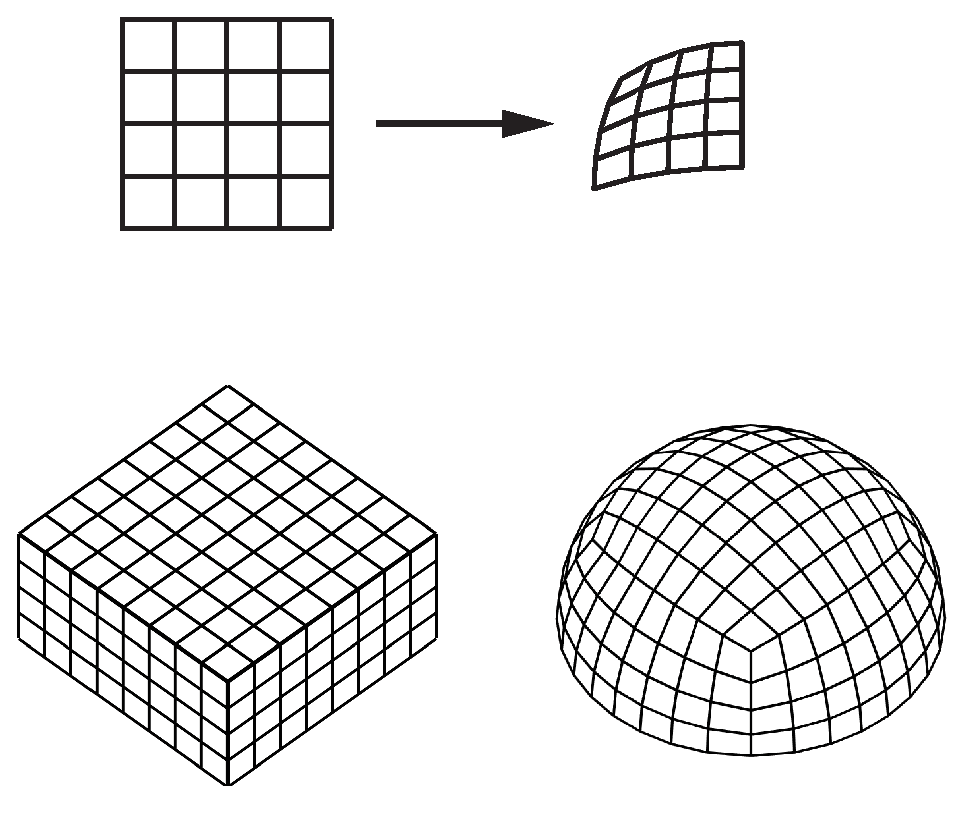
\includegraphics[width=0.65\textwidth]{mapping}
    \caption{A schematic description of the mapping from a rectilinear patch to a patch on the sphere surface (top). The entire mapping from a half-cube to a hemisphere (bottom). }
    \label{fig:mapping}
\end{figure}